\documentclass[oneside,a4paper]{article}

% ========== Preamble (packages, definitions etc.) ==========

\usepackage[utf8]{inputenc}
\usepackage[english]{babel}
\usepackage{graphicx}
\usepackage{xcolor}
\usepackage{amsmath, amsthm, amssymb}
\usepackage{csquotes}
\usepackage{hyperref}
\usepackage{listings}
\usepackage{lmodern}
\usepackage[explicit]{titlesec}
\usepackage{color}
\usepackage{listings}
\lstset{
    breaklines=true,
    basicstyle=\tt\normalsize,
    keywordstyle=\color{blue},
    identifierstyle=\color{magenta},
    frame = single
} 
%\usepackage[backend=bibtex,style=abbrv]{biblatex}
% Please add the following required packages to your document preamble:
\usepackage{booktabs}
\usepackage[normalem]{ulem}
\useunder{\uline}{\ul}{}
\newcommand{\todo}[1]{{\color{blue}#1}}  % show to-do items in blue
\setlength{\parskip}{\baselineskip}
\usepackage[activate={true,nocompatibility},
            final,
            tracking=true,
            kerning=true,
            %spacing=nonfrench,
            factor=1100,
            stretch=10,
            shrink=10,
            nopatch=eqnum]{microtype}
%\hypersetup{
%    pdftitle={},
%    bookmarks=true,
%    pdfpagemode=FullScreen,
%}

\newcounter{questionnum} \setcounter{questionnum}{0}
%\newcommand{\question}[1]{%
%  \refstepcounter{questionnum}%
%  \paragraph{Question~\arabic{questionnum}:}{\emph{#1}}}

\newcommand\filltoend{\leavevmode{\unskip
  \leaders\hrule height.5ex depth\dimexpr-.5ex+0.4pt\hfill\hbox{}%
  \parfillskip=0pt\endgraf}}

\newcommand{\problem}[2]{%
	\vspace{-0.7em}
	\hspace{0.02\textwidth}
	\begin{minipage}[t][][b]{0.95\textwidth}
		{\bf \hspace{-0.015\textwidth}\makebox[7.5em][l]{{#1} ~~\filltoend}}%
		\hspace{1.2mm}{\it #2}%
	\end{minipage}
}

\definecolor{redbg}{RGB}{235, 214, 214}
\definecolor{Red}{RGB}{163, 25, 25}
\definecolor{Black}{RGB}{0, 0, 0}


\titleformat{\section}
  {\normalfont\LARGE\bfseries}
  {}
  {0em}
  {\colorbox{redbg}{\parbox{\dimexpr\textwidth-2\fboxsep\relax}{\textcolor{Red}{\thesection\quad#1}}}}

\titleformat{\subsection}
  {\normalfont\large\bfseries\color{Black}}
  {\thesubsection}
  {1em}
  {#1}
  [{\titlerule[0.8pt]}]

\titlespacing\subsection{0pt}{12pt plus 4pt minus 2pt}{0pt plus 2pt minus 2pt}

\def\email#1{{\tt#1}}

\lstset{ % Set the default style for code listings
	numbers=left,
	numberstyle=\scriptsize,
	numbersep=8pt,
	basicstyle=\scriptsize\ttfamily,
	keywordstyle=\color{blue},
	stringstyle=\color{red},
	commentstyle=\color{green!70!black},
	breaklines=true,
	frame=single,
	language=bash,
	tabsize=4,
	showstringspaces=false
}
\usepackage{svg}
\usepackage{float}
\usepackage[margin=2cm]{geometry}
\usepackage{pdfpages}
\usepackage[title]{appendix}
\usepackage{indentfirst}
\usepackage{caption, subcaption}
\usepackage{enumitem}


% ========== Title page ==========

\title{
	
\includegraphics[width=0.6\textwidth]{UU_logo.pdf}\\[1em]
	Computer-Assisted Image Analysis I - 1TD396\\[1em]
	Computer Exercise 4\\[3em]
}

\author{
	Jyong-Jhih Lin, \and Linus Falk, \and Niklas Kostrzewa, \and Teng-Sung Yu
	%
}

\date{December 01, 2022}

\begin{document}

\maketitle
\thispagestyle{empty} % Removes page number for front page
\pagebreak

% ========== Document contents ==========
\section{Classification basics}



\subsection*{Q1 Are the two classes possible to separate by using either the x or y coordinate as a single feature? Explain why or why not}
\noindent No there seems to be some correlation between the x and y variable. Splitting the two classes would need a line of the sort : y = kx+m.

\begin{figure}[ht!]
\centering
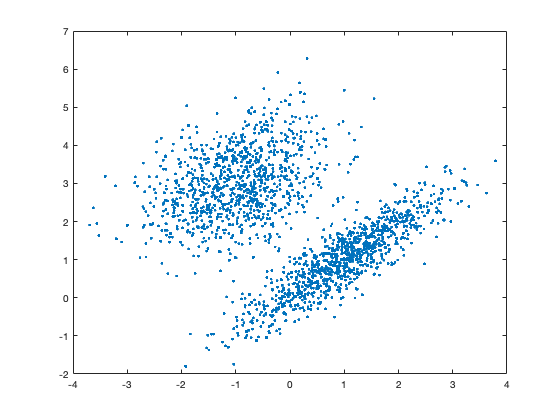
\includegraphics[width=100mm]{figures/Q1.png}
\caption{Q1}
\label{fig:Q1}
\end{figure}

\subsection*{Q2 Does multiple thresholding give a successful classification of the three classes? Explain why or why not.}
\noindent No since the hand and ring have approximately the same intensity. This makes it very difficult or impossible to segment it by using the intensity only.


\begin{figure}[ht!]
\centering
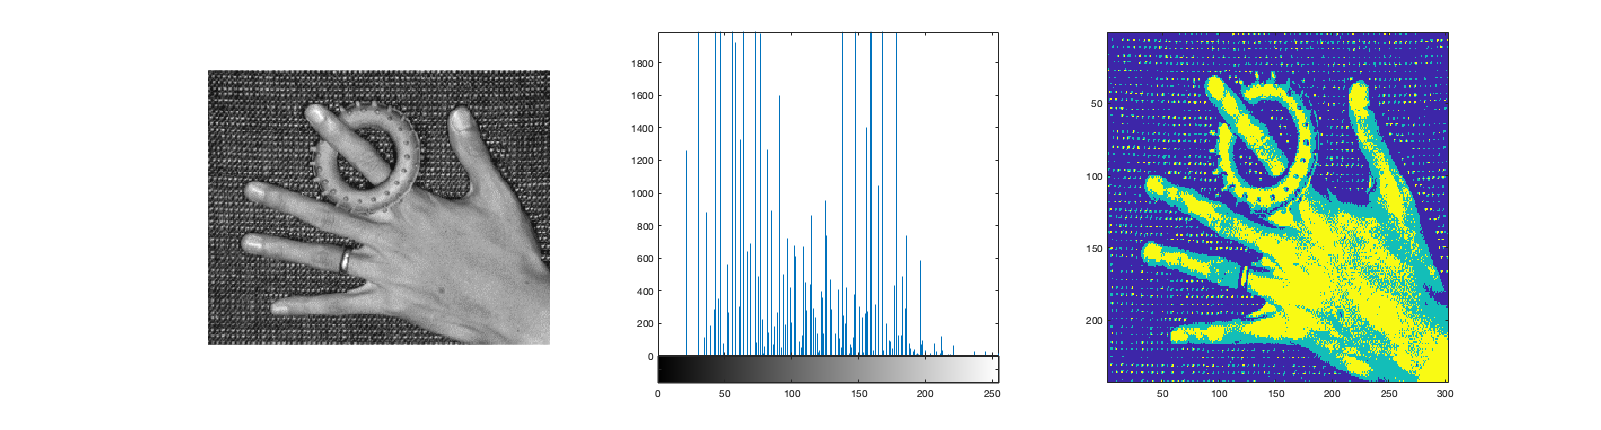
\includegraphics[width=130mm]{figures/Q2.png}
\caption{Q2}
\label{fig:Q2}
\end{figure}

\begin{lstlisting}[language=MATLAB]
figure(2);
I = imread("lab4-codes-images/handBW.pnm");
subplot(1,3,1);  
imshow(I);
subplot(1,3,2);
imhist(I);

t1 = 120;
t2 = 160; 

subplot(1,3,3);
mtresh(I,t1,t2)
\end{lstlisting}

\subsection*{Q3 MATLAB’s classify function uses Linear Discriminant Analysis (LDA) as default. What assumptions are made on the data by an LDA classifier? Also, what makes a classifier linear?}
\noindent LDA assumes that the sampled features/measurements are Gaussian distributed and the covariance of the measurements are identical across different classes. A linear classifier is linear when the decision boundary is linear in the input space. 


\subsection*{Q4 Have the results improved using classification compared to threshold? Is the classification more successful in the case with the gray scale image or single bands? Explain. Does it improve the classification to incorporate pairs of bands or the full RGB information? Discuss. Show your results from gray scale classification, one pair of features and full RGB classification.}
\noindent The results have improved using the classification compared to only using threshold of the histogram. The classification is better on one channel of the RGB image then the grey scale image. In the one channel RGB case we can choose which channel that gives the best separation of the object and and background and makes the classification simpler. A way to think about it is that when choosing one of the band is like taking the photo with a colored filter in front of the camera lens, some colors are enhanced and other are not. The classification improves adding one band but is best when incorporating all bands. This suggest that we have useful data in all bands that make the classification easier to do. This depends on the image and the result can change depending on the content of the image. In this case is the classification done by the color of the object so its quite clear that the more color information we use will improve the result. 

\begin{figure}[ht!]
\centering
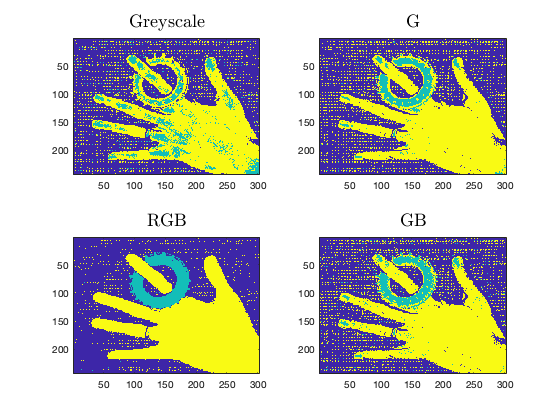
\includegraphics[width=130mm]{figures/Q4.png}
\caption{Q4}
\label{fig:Q4}
\end{figure}

\begin{lstlisting}[language=MATLAB]
figure(7);
I3(:,:,1) = G;
I3(:,:,2) = B;
I4(:,:,1) = G;
[data,class] = create_training_data(I3,label_im);
scatterplot2D(data,class);

[data,class] = create_training_data(I,label_im);
Itest = im2testdata(I); % Reshape the image before classification
C = classify(double(Itest),double(data),double(class)); % Train classifier and classify the data
ImC1 = class2im(C,size(I,1),size(I,2)); % Reshape the classification to an image

[data,class] = create_training_data(I4,label_im);
Itest = im2testdata(I4); % Reshape the image before classification
C = classify(double(Itest),double(data),double(class)); % Train classifier and classify the data
ImC2 = class2im(C,size(I4,1),size(I4,2)); % Reshape the classification to an image

[data,class] = create_training_data(I2,label_im);
Itest = im2testdata(I2); % Reshape the image before classification
C = classify(double(Itest),double(data),double(class)); % Train classifier and classify the data
ImC3 = class2im(C,size(I2,1),size(I2,2)); % Reshape the classification to an image

[data,class] = create_training_data(I3,label_im);
Itest = im2testdata(I3); % Reshape the image before classification
C = classify(double(Itest),double(data),double(class)); % Train classifier and classify the data
ImC4 = class2im(C,size(I3,1),size(I3,2)); % Reshape the classification to an image

figure(9);
subplot(2,2,1)
imagesc(ImC1);
title('Greyscale','Interpreter','latex', 'fontsize',18);
subplot(2,2,2)
imagesc(ImC2);
title('G','Interpreter','latex', 'fontsize',18);
subplot(2,2,3)
imagesc(ImC3); 
title('RGB','Interpreter','latex', 'fontsize',18);
subplot(2,2,4)
imagesc(ImC4); 
title('GB','Interpreter','latex', 'fontsize',18);
\end{lstlisting}


\section{Classification of multispectral data}

\subsection*{Q5 Which bands are you using for your classification? What classifier are you using? Which classes are possible to separate in a good way? Illustrate with images and scatterplots. Show images from your classification result and compare with classification using all bands. Discuss your results.}

\noindent Using the LDA since it was difficult to pick out a good training patch of the image that didn't result in non positive definite covariance matrix which is a requirement for QDA. The different band from the landsat 7 data is useful for different kind of classifications. In table: REF we can see  recommended classification for each band. From this we conclude that 1, 2 and 4 should be suitable to detect the labels: agriculture, woods, city, and water. The training data is presented in figure: REF. Investigating the training data with scatter plots we can conclude that it should be possible to separate this classes with LDA. 


\begin{table}[ht!]
\begin{tabular}{@{}lll@{}}
\toprule
\textbf{Band} & \textbf{Wavelength} & \textbf{Useful for mapping}                                                   \\ \midrule
Band 1        & 0.45-0.52           & Bathymetric mapping, distinguishing soil from vegetation ...                  \\
Band 2        & 0.52-0.60           & Emphasizes peak vegetation, which is useful for assessing plant vigor         \\
Band 3        & 0.63-0.69           & Discriminates vegetation slopes                                               \\
Band 4        & 0.77-0.90           & Emphasizes biomass content and shorelines                                     \\
Band 5        & 1.55-1.75           & Discriminates moisture content of soil and vegetation; penetrates thin clouds \\
Band 6        & 10.40-12.50         & Thermal mapping and estimated soil moisture                                   \\
Band 7        & 2.09-2.35           & Hydrothermally altered rocks associated with mineral deposits                 \\ \bottomrule
\end{tabular}
\caption{Source: \url{https://www.usgs.gov/faqs/what-are-best-landsat-spectral-bands-use-my-research\#faq}}
\end{table}



\begin{figure}[ht!]
\centering
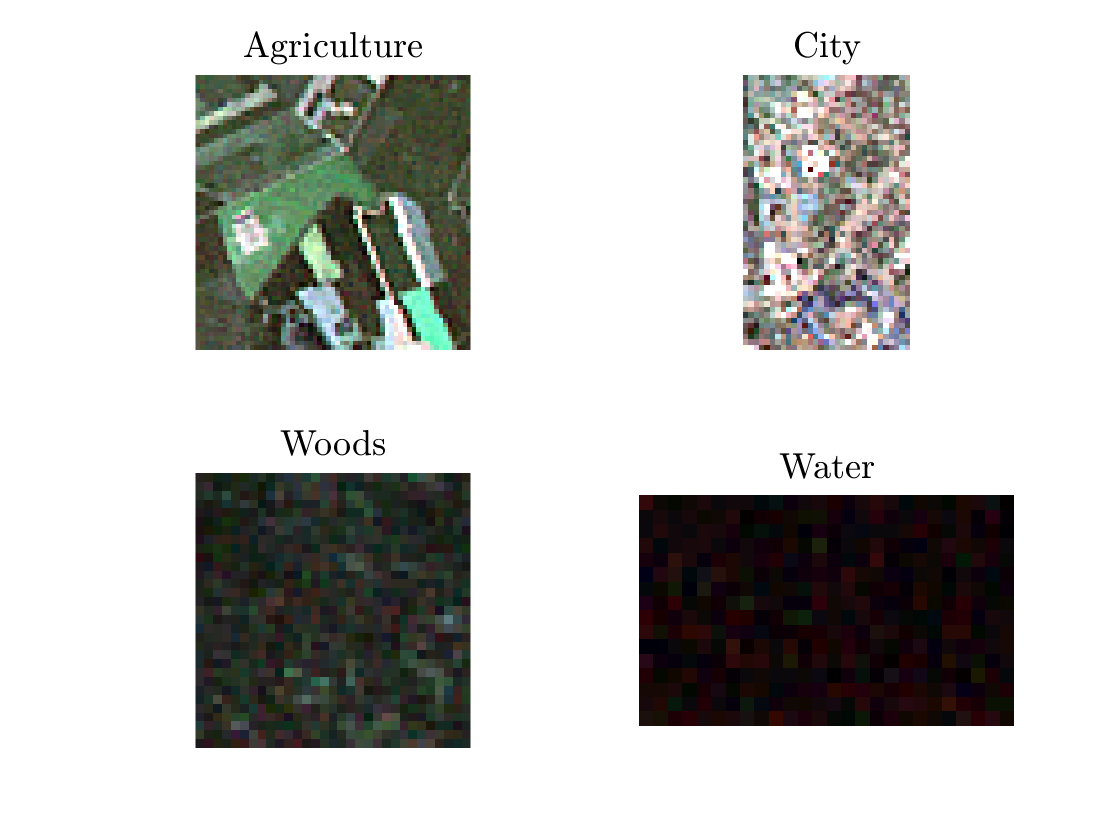
\includegraphics[width=60mm]{figures/training.png}
\caption{Training data in band [1,2,3]}
\label{fig:Q5train}
\end{figure}

\newpage




\begin{figure}[ht!]
\centering
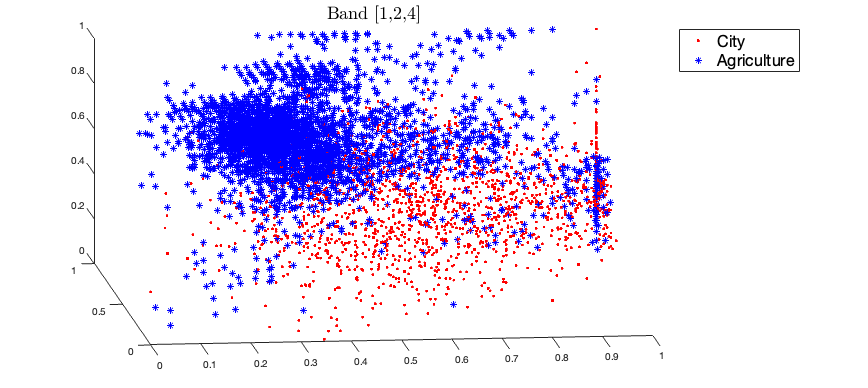
\includegraphics[width=140mm]{figures/Q5.png}
\caption{Scatter plot of band [1,2,4] in training data}
\label{fig:Q5}
\end{figure}

\begin{figure}[ht!]
\centering
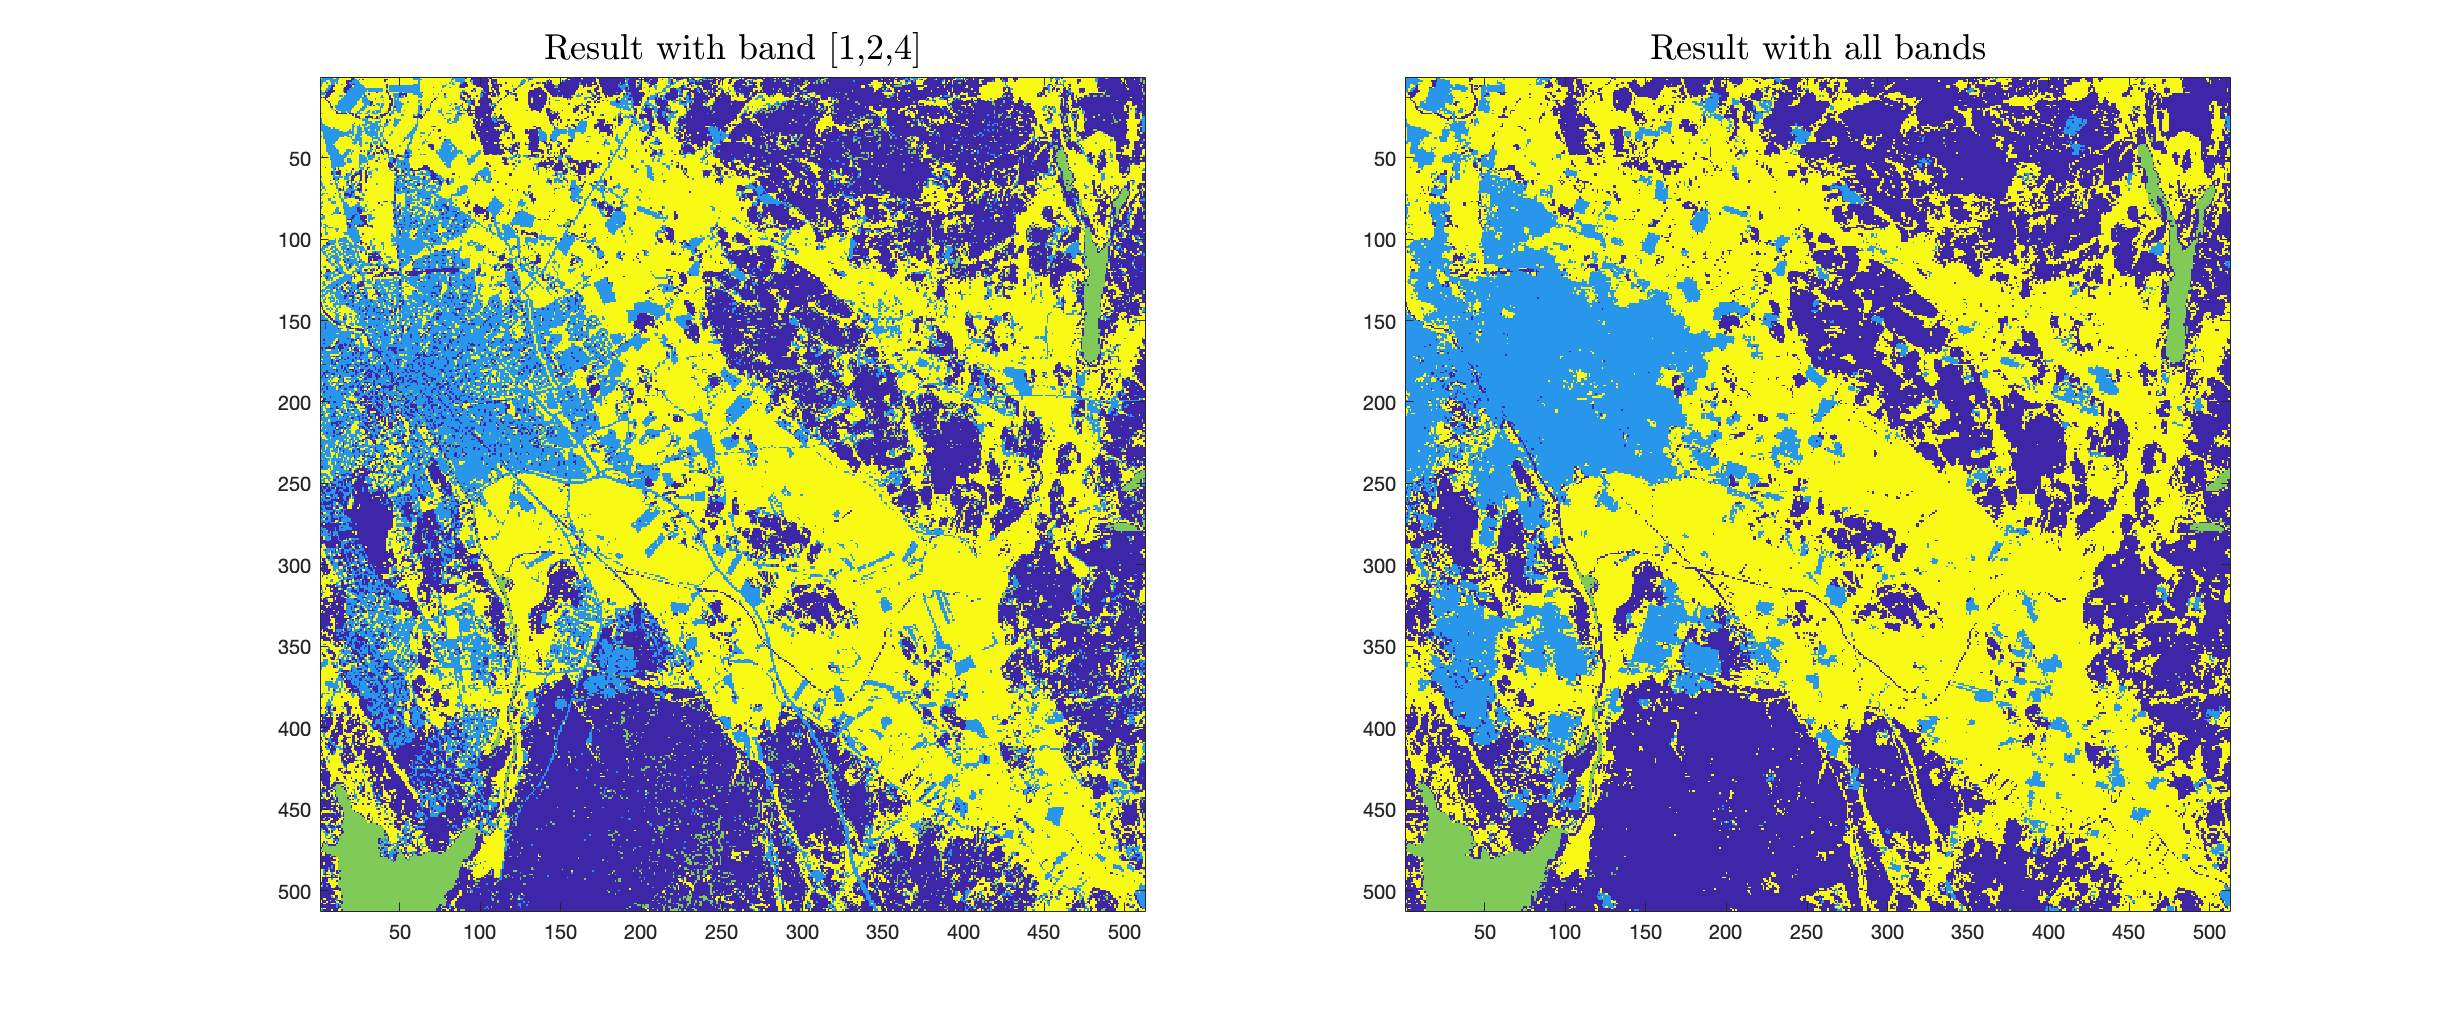
\includegraphics[width=150mm]{figures/result.png}
\caption{Result with band [1,2,4] and all}
\label{fig:result}
\end{figure}

\subsection*{Q6 Is there any reason not to include all bands if they are not needed to separate the
classes?}
\noindent Using all bands creates a resolution problem  since band 6 is into the infrared and have a resolution of approximately half of the other bands, we therefore lose details when including this. When using this band to distinguish for example building in the city we run into problem. Comparing the results from all band with band 1,2 and 4 we can see that in the later case we can distinguish vegetation in the city between the building that we cant with all bands.  
%https://www.usgs.gov/faqs/what-are-band-designations-landsat-satellites
\newpage


\begin{lstlisting}[language=MATLAB]
load lab4-codes-images/landsat_data.mat

T = zeros(512,512); % Create an empty image
T(450:480,140:170) = 1; %woods
T(130:180,50:80) = 2; %city
T(490:505,25:50) = 3; %water
T(290:350,340:400) = 4; %agriculture

agri = (landsat_data(290:350,340:400,[1,2,4])./255);
city = (landsat_data(130:180,50:80,[1,2,4])./255);
water = (landsat_data(490:505,25:50,[1,2,4])./255);
woods = (landsat_data(450:480,140:170,[1,2,4])./255);

figure(999);
subplot(2,2,1)
imshow(agri);
title('Agriculture','Interpreter','latex', 'fontsize',18);
subplot(2,2,2)
imshow(city)
title('City','Interpreter','latex', 'fontsize',18);
subplot(2,2,3)
imshow(woods)
title('Woods','Interpreter','latex', 'fontsize',18);
subplot(2,2,4)
imshow(water)
title('Water','Interpreter','latex', 'fontsize',18);


%imtool(landsat_data(:,:,[1,2,3])./255)

figure(2);
p1 = plot3(city(:,:,1),city(:,:,2),city(:,:,3),'.', 'Color','red');
hold on;
p2 = plot3(agri(:,:,1),agri(:,:,2),agri(:,:,3),'*', 'Color','blue')
h = [p1(1),p2(1)];
legend(h, 'City', 'Agriculture', 'fontsize', 16)
title('Band [1,2,4]','Interpreter','latex', 'fontsize',18)

%[2,5,6]
%[1,4,2] the best
I = (landsat_data(:,:,[1,4,2])./255); 
[data,class] = create_training_data(I,T);
Itest = im2testdata(I); % Reshape the image before classification
C = classify(double(Itest),double(data),double(class),'linear'); % Train classifier and classify the data
ImC1 = class2im(C,size(I,1),size(I,2)); % Reshape the classification to an image

I = (landsat_data(:,:,:)./255); 
[data,class] = create_training_data(I,T);
Itest = im2testdata(I); % Reshape the image before classification
C = classify(double(Itest),double(data),double(class),'linear'); % Train classifier and classify the data
ImC2 = class2im(C,size(I,1),size(I,2)); % Reshape the classification to an image



figure(3)
subplot(1,2,1)
imagesc(ImC1);
title('Result with band [1,2,4]','Interpreter','latex', 'fontsize',18)
subplot(1,2,2)
imagesc(ImC2);
title('Result with all bands','Interpreter','latex', 'fontsize',18)

\end{lstlisting}

\newpage 

\section{Classification based on texture}

\subsection*{Q7 Which ”offset” value did you use for the co-occurrence matrix? Plot uniformity and entropy for all the objects. You should have a plot similar to Figure 3. Using entropy and uniformity, say which objects are outliers and should be removed from the sequence. Why?}

\noindent We used offset [2 0] for the co-occurrence matrix. This means that the gray-level co-occurrence matrix is calculated in the vertical proximity of the pixel. In this example we could use one parameter to remove the wrong classifications. Entropy is a measure of variability in images while uniformity gives a maximum for image with just one gray value. Setting a threshold of 3e7 for the uniformity for an example. The virus cutouts are less uniform and gives a lower value then the background and therefore yields a lower Uniformity value. We can clearly see a group that sits higher up in the plot that we classify as outliers. Additionally could one cutout (nr 14 in fig \ref{fig:Q7bef}) be removed as outlier using entropy as a measurement since it doesn't share that bright part as any of the other virus cutouts. 



\begin{figure}[ht!]
\centering
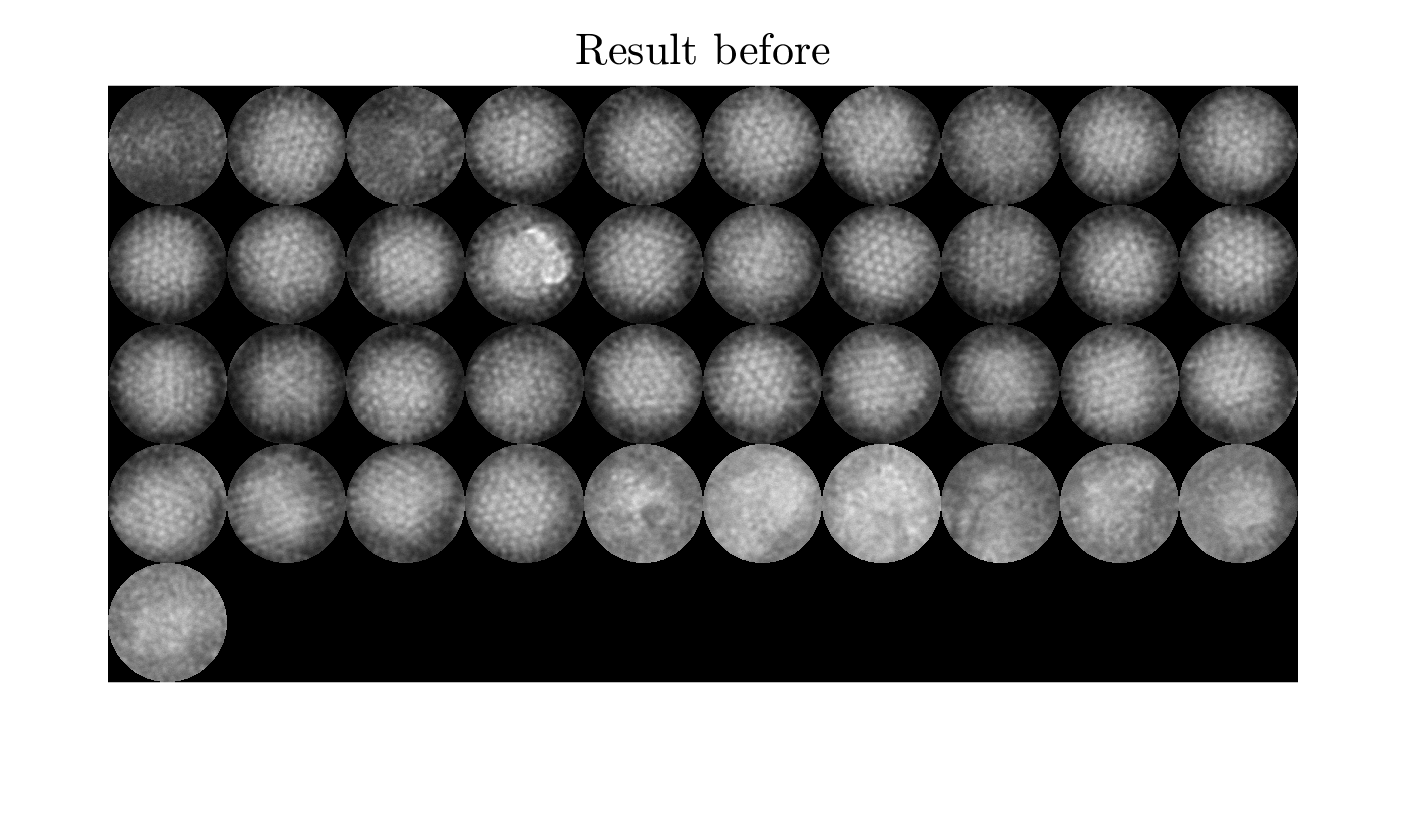
\includegraphics[width=140mm]{figures/Q7_before.png}
\caption{Result before}
\label{fig:Q7bef}
\end{figure}

\begin{figure}[ht!]
\centering
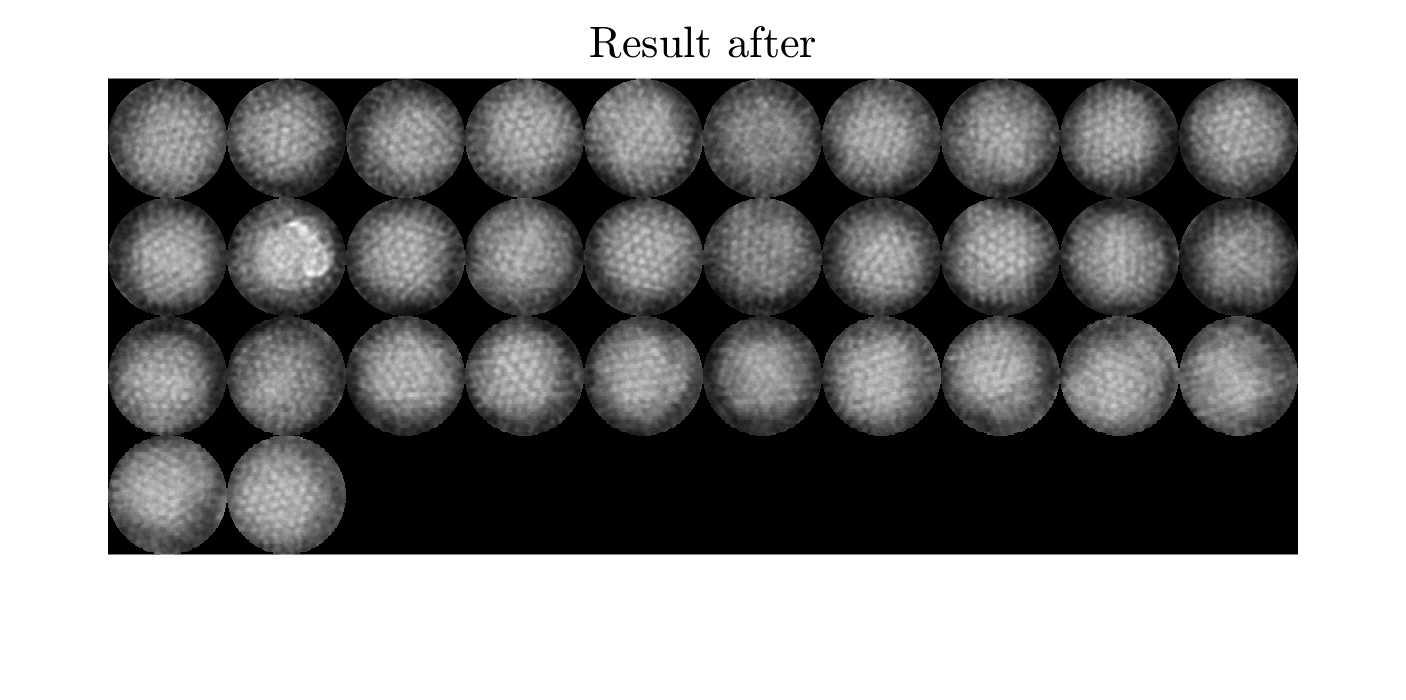
\includegraphics[width=140mm]{figures/q7after.png}
\caption{Result after}
\label{fig:Q7after}
\end{figure}

\newpage

\begin{figure}[ht!]
\centering
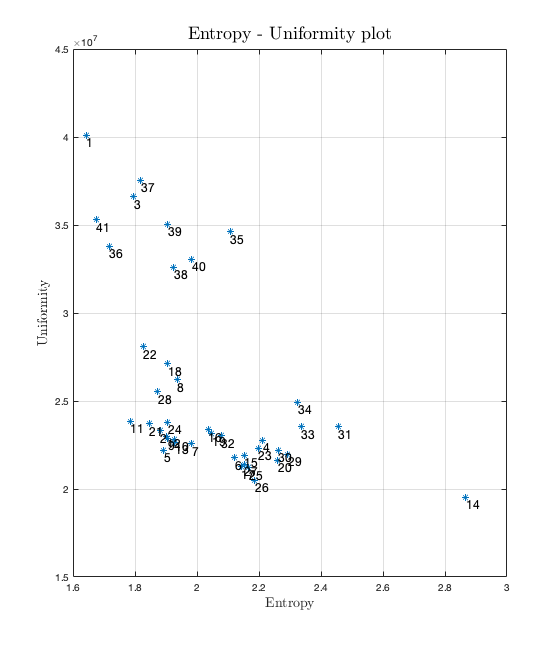
\includegraphics[width=140mm]{figures/uniformity_entropy.png}
\caption{Entropy and uniformity plot}
\label{fig:entro}
\end{figure}

\begin{lstlisting}[language=MATLAB]
% Place for your own texture analysis. 
forplot = zeros(41,2);
for i=1:41    
    A = graycomatrix(cutouts{i},'Offset',[2 0]);
    forplot(i,2) = sum(A(:).^2);%sum(A(A~=0).^2);             %Uniformity
    A = mat2gray(A);
    forplot(i,1) = entropy(A); %-sum(A(A~=0).*log2(A(A~=0))); %Entropy
    
end

labels = {'1','2','3','4','5','6','7','8','9','10','11','12','13','14','15','16','17','18','19','20','21','22','23','24','25','26','27','28','29','30','31','32','33','34','35','36','37','38','39','40','41'};
figure(100)

plot(forplot(:,1),forplot(:,2),'*')
text(forplot(:,1),forplot(:,2),labels,'VerticalAlignment','top','HorizontalAlignment','left', 'FontSize',12)
title('Entropy - Uniformity plot','Interpreter','latex', 'fontsize',18);
xlabel('Entropy','Interpreter','latex', 'fontsize',14);
ylabel('Uniformity','Interpreter','latex', 'fontsize',14);
grid on; 

for i=1:41    
    A = graycomatrix(cutouts{i},'Offset',[1 1]);
    if  sum(A(A~=0).^2) > 3e7
        cutouts{i} = [];
    end
    forplot(i,2) = sum(A(A~=0).^2);
end

 cutouts = cutouts(~cellfun('isempty',cutouts));

%% Collect all cutouts in an image

imagesPerRow = 10;
cols = imagesPerRow;
rows = ceil(size(cutouts,2) / cols);

objectMap = uint8(zeros(size(mask).*[rows cols]));
counter = 1;

for i = 1 : rows
    for j = 1 : cols
        if counter <= size(cutouts,2)
            objectMap((i-1)*d+1:(i-1)*d+d,(j-1)*d+1:(j-1)*d+d) = cutouts{counter}(:,:);
            counter = counter + 1;
        end
    end    
end

figure('name','Cutouts of segmented objects');imshow(objectMap);
title('Result after','Interpreter','latex', 'fontsize',22);

\end{lstlisting}

% Delete this section if you have no plot to submit.
% Change the size of the figure by changing the value in [width=300pt]

% Putting \autoref{fig:my_figure} in your text will refer to the corresponding figure label.
% Eg.: "\autoref{fig:my_figure} clearly shows that the large circle is larger than the small box."
% Read more about autoref here https://en.wikibooks.org/wiki/LaTeX/Labels_and_Cross-referencing#autoref

%\bibliographystyle{apalike}
%\bibliographystyle{abbrv}
%\bibliography{bibliography}

\end{document}